\documentclass[a4paper,10pt]{article}

\usepackage{graphicx}
\usepackage[utf8]{inputenc}
\usepackage[T1]{fontenc}
\usepackage{wrapfig}

\usepackage{hyperref}
\setlength{\parindent}{10pt}
\setlength{\parskip}{1.5mm}
\usepackage{geometry}
\geometry{margin=1.25cm}
\addtolength{\textheight}{-1.5cm}
\setlength{\headheight}{32pt}

\usepackage{amsfonts, amstext, color,
	ifthen, fancybox, multirow, fancyhdr, pgf, tikz,%
	colortbl, array, tabularx
}

\definecolor{bgcode}{rgb}{0.95,0.95,0.95}

\usepackage{url}

\usepackage[french]{babel}
\selectlanguage{french}

%partie concernant la gestion des entêtes
\usepackage{fancyhdr}
\pagestyle{fancy}
\usepackage{lastpage}
\renewcommand\headrulewidth{1pt}
\fancyhead[L]{Interface Homme-Machine Android}
\fancyhead[R]{Université de Poitiers}
\renewcommand\footrulewidth{1pt}
\fancyfoot[L]{Département d'Informatique}
\fancyfoot[C]{\textbf{\thepage/\pageref{LastPage}}}
\fancyfoot[R]{année 2022-2023}
%fin

\usepackage{enumitem}

\usepackage{listings}

\usepackage{version}
\usepackage{tcolorbox}

\newcounter{Exercice}
\newcommand{\Exercice}[1]{\refstepcounter{Exercice}%
	\ \vspace{0mm} \\ \hspace{0.8cm}%
	\noindent \hspace*{0.5cm} {\bf Question \theExercice :} #1 \vspace{-13mm} \\ %
	\subparagraph*{}%
}

\lstset{language=Caml,basicstyle=\normalsize\tt,keywordstyle=\ttfamily\bfseries\underbar,%
	commentstyle=\normalsize, extendedchars=true, fontadjust=true, columns = flexible, flexiblecolumns=true,
	linewidth=.975\linewidth, backgroundcolor=\color{bgcode}, frame=tlrb, xleftmargin=1cm}

\lstnewenvironment{ocamlcode}
{\lstset{language=Caml,basicstyle=\normalsize\tt,keywordstyle=\ttfamily\bfseries\underbar,%
		commentstyle=\normalsize, extendedchars=true, fontadjust=true, columns = flexible, flexiblecolumns=true,
		linewidth=.975\linewidth, backgroundcolor=\color{bgcode}, frame=tlrb, xleftmargin=1cm,
		literate={à}{{\`a}}1 {è}{{\`e}}1 {é}{{\'e}}1 {ê}{{\^e}}1,
	}}%, framexleftmargin=5mm,frame=box}}
{}

\lstnewenvironment{fsharp}
{\lstset{language=Caml,basicstyle=\normalsize\tt,keywordstyle=\ttfamily\bfseries\underbar,%
		commentstyle=\normalsize, extendedchars=true, fontadjust=true, columns = flexible, flexiblecolumns=true,
		linewidth=.975\linewidth, backgroundcolor=\color{bgcode}, frame=tlrb, xleftmargin=1cm,
		literate={à}{{\`a}}1 {è}{{\`e}}1 {é}{{\'e}}1 {ê}{{\^e}}1 {ç}{{\c c}}1,
}}%, framexleftmargin=5mm,frame=box}}
{}

\lstnewenvironment{javasansbord}
{\lstset{language=Java,basicstyle=\normalsize\tt,keywordstyle=\ttfamily\bfseries\underbar,%
		commentstyle=\normalsize, extendedchars=true, fontadjust=true, columns = flexible, flexiblecolumns=true,
		linewidth=.975\linewidth,frame=,backgroundcolor=,xleftmargin=0cm,
		literate={à}{{\`a}}1 {è}{{\`e}}1 {é}{{\'e}}1 {ê}{{\^e}}1 {ç}{{\c c}}1,
}}%, framexleftmargin=5mm,frame=box}}
{}

\lstnewenvironment{java}
{\lstset{language=Java,basicstyle=\normalsize\tt,keywordstyle=\ttfamily\bfseries\underbar,%
		commentstyle=\normalsize, extendedchars=true, fontadjust=true, columns = flexible, flexiblecolumns=true,
		linewidth=.975\linewidth, backgroundcolor=\color{bgcode}, frame=tlrb, xleftmargin=1cm,
		literate={à}{{\`a}}1 {è}{{\`e}}1 {é}{{\'e}}1 {ê}{{\^e}}1 {ç}{{\c c}}1,
}}%, framexleftmargin=5mm,frame=box}}
{}

\newboolean{versionenseignant}
%%%%%%%%%%%%%%%%%%%%%%%%%%%%%%%%%%%%%%%%%%%%%%%%%%%%%%%%%%%%%%%%%%%%%%%%%%%%%%%%%%%%%%%%%%%%%%%%%%%%%%%%
%__     __            _
%\ \   / /__ _ __ ___(_) ___  _ __
% \ \ / / _ \ '__/ __| |/ _ \| '_ \
%  \ V /  __/ |  \__ \ | (_) | | | |
%   \_/ \___|_|  |___/_|\___/|_| |_|
% _____                _                         _
%| ____|_ __  ___  ___(_) __ _ _ __   __ _ _ __ | |_
%|  _| | '_ \/ __|/ _ \ |/ _` | '_ \ / _` | '_ \| __|
%| |___| | | \__ \  __/ | (_| | | | | (_| | | | | |_
%|_____|_| |_|___/\___|_|\__, |_| |_|\__,_|_| |_|\__|
%                        |___/ 
%% modifiez le booleen ci-dessous pour generer la version enseignant ou etudiant
%% ===> true = version enseignant
%% ===> false = version etudiant
\setboolean{versionenseignant}{false}
%%%%%%%%%%%%%%%%%%%%%%%%%%%%%%%%%%%%%%%%%%%%%%%%%%%%%%%%%%%%%%%%%%%%%%%%%%%%%%%%%%%%%%%%%%%%%%%%%%%%%%%%
% \includeversion{ensnote}
%\excludeversion{ensnote}
\ifthenelse{\boolean{versionenseignant}}{\includeversion{ensnote}}{\excludeversion{ensnote}}

\tcbuselibrary{breakable}


\newenvironment{solution}%
{\begin{tcolorbox}[breakable,colback=red!5!white,colframe=red!75!black,title=Solution]}%
{\end{tcolorbox}}

%\tcblower

\newenvironment{info}%
{\begin{tcolorbox}[breakable,colback=green!5!white,colframe=green!75!black,title=Information]}%
{\end{tcolorbox}}


\newenvironment{attention}%
{\begin{tcolorbox}[breakable,colback=green!25!white,colframe=red!55!black,title=Attention]}%
{\end{tcolorbox}}


\newenvironment{boxcode}%
{\begin{tcolorbox}[breakable,colback=gray!5!white,colframe=black]}%
	{\end{tcolorbox}}
	
	
\begin{document}
	


\title{\vspace*{-1cm}Manipulation des layouts}
\author{\vspace*{-1.5cm}Interface Homme-Machine: Unity
\begin{ensnote}
	(Version enseignant)
\end{ensnote}
}
\date{\vspace*{-1.5cm}version 1}
\maketitle
\thispagestyle{fancy}

Voici les objectifs de ce sujet:
\begin{itemize}
	\item continuer à manipuler l'IDE \texttt{Unity};
	\item continuer la création d'un \textit{widget} complexe;
	\item exploiter les mécaniques vues précédemment;
	\item utiliser les \texttt{Layouts}.
\end{itemize}


%\begin{attention}
%	Le sujet ce fait en deux étapes. Avec une proposition notée de votre interface au bout de 2h (si vous avez fini avant la \textit{deadline} rien ne vous empêche de continuer)!
%	
%	N'oubliez pas d'utiliser les bons réflexes de tout développeur:
%	\begin{itemize}
%		\item Le système de log très bien fait sous Android
%		\item Le mode débogue qui vous permet de voir les valeurs des variables pendant 
%	\end{itemize}
%\end{attention}

\section{Description générale du TP}

La fois précédente, nous avons réalisé nos premiers widgets complexes en exploitant l'agrégation de plusieurs widgets de base. Nous avons en particulier manipulé le système d'ancre que propose \texttt{Unity} pour placer les objets de façon relative.

Ici, nous allons voir une autre méthode un peu plus coûteuse mais offrant une plus grande puissance en terme de placement et qui reprend les points que vous avez étudié dans les années précédentes en IHM: les mises en page (\texttt{layout}). La documentation est présente ici: \url{https://docs.unity3d.com/Packages/com.unity.ugui@1.0/manual/UIAutoLayout.html}

\subsection*{Composants basiques}

\begin{itemize}
	  \item Tester les propriétés du  composant \texttt{Content Size Fitter} sur un \texttt{GameObject} de type \texttt{Text} ou \texttt{Image}.
	  
	  \item Faites de même pour le composant \texttt{Aspect Ratio Filter}. Pour bien distinguer les effets de chaque composant, il est recommandé d'en associer un seul à la fois au \texttt{GameObject}.
\end{itemize}

\section{Présentation des outils de mise en pages en Unity UI}

Il est conseillé de lire en détail la documentation citée plus haut pour bien comprendre les aspects et tous les détails. Voici le résumé des points clés:
\begin{itemize}
	\item Il y a deux types de composants dédiés à la mise en page.
	\item Les \textit{conteneurs} ou \texttt{Layout Group} contrôlent le comportement des widgets fils (enchaînement horizontal, enchaînement vertical ou sous forme de grille, \ldots)
\begin{center}
	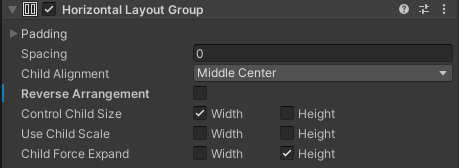
\includegraphics[width=0.6\linewidth]{rc/ui_layout_group_horiz}
\end{center}	
	\item Les composants \textit{éléments} ou \texttt{Layout Element} qui indiquent leur présence de mise en page.
\begin{center}
	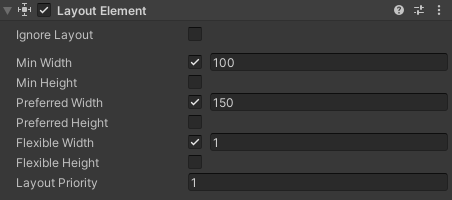
\includegraphics[width=0.6\linewidth]{rc/ui_layout_element}
\end{center}
\end{itemize}

Ainsi, chaque conteneur peut avoir des paramétrages différents qui vont faire évoluer les éléments selon les contraintes. Vous ferez attention à certains paramètres qui peuvent forcer le redimensionnement des widgets éléments sans les consulter même si leur taille n'était pas voulue. Vous ferez aussi attention aux éléments qui doivent activer la flexibilité des dimensions voulues pour agrandir dans cette direction (une valeur de 1 peut être suffisante pour indiquer un degré de liberté).

\subsection*{Tests}

\begin{enumerate}
	\item Dans un premier temps, tester les conteneurs \texttt{Horizontal Layout Group}, \texttt{Vertical Layout Group} et \texttt{Grid Layout Group} \textbf{sans} ajouter de composant \texttt{Layout Element} aux enfants des groupes.
	\item Associer ensuite des \texttt{Layout Element} aux enfants des groupes et tester les conteneurs.
\end{enumerate}

\section{Widget: ComplexSlider - le retour en joli}

Refaites le widget \texttt{ComplexSlider} (soit sous un autre nom, soit après avoir fait une sauvegarde de votre ancien projet/widget). Pour obtenir un affichage joli, peu importe la largeur que vous donnerez à votre widget, pourvu que le \texttt{Slider} prenne la plus grande place.

Veillez à ce que le widget contenant la valeur numérique ne soit pas modifiable directement par l'utilisateur.

\begin{center}
	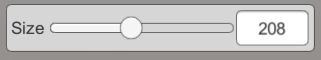
\includegraphics[width=0.6\linewidth]{rc/ui_complexslider_layout}

	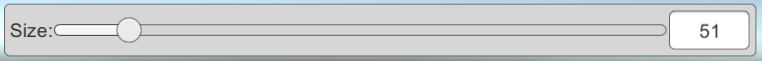
\includegraphics[width=0.8\linewidth]{rc/ui_complexslider_layout_v2}
	
\end{center}


\section{Widget: Spinner}

Réalisez le widget du \texttt{Spinner} qui consiste à contrôler les évolutions d'un nombre via deux boutons regroupés en bout de ligne. 

La valeur de l'incrément (positif ou négatif) sera laissé au choix de l'utilisateur. 

\begin{center}
	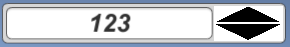
\includegraphics[width=0.6\linewidth]{rc/ui_spinner_layout}
\end{center}

Le widget doit être fonctionnel, mais vous pouvez bien sûr changer/adapter selon vos souhaits le coté esthétique du widget.
De nouveau, vérifiez que le widget contenant la valeur numérique ne soit pas modifiable directement par l'utilisateur.

\section{Aspects avancés sur le système d'événement souris}

Le système événementiel est en cours de modification, mais nous présentons ici une mécanique pour interagir avec des événements particuliers. Pour cela, consultez le lien suivant qui donne les événements supportés \url{https://docs.unity3d.com/Packages/com.unity.ugui@1.0/manual/SupportedEvents.html}. Nous vous proposons un petit exercice sous forme de tutoriel:
\begin{itemize}
	\item Dans un nouveau projet ou une nouvelle \texttt{Scene}\footnote{Dans ce dernier cas, ajouter dans chaque scène un bouton pour permuter entre les scènes.}, ajoutez un \texttt{Panel} occupant l'entièreté du \texttt{Canvas}.
	\item Modifiez la couleur du \texttt{Panel} pour qu'il soit entièrement transparent.
	\item Ajoutez un nouveau script.
	\item Au début du fichier script, ajoutez la ligne \lstinline|using UnityEngine.EventSystems;|.
	\item Faire hériter le script avec les événements voulus (cf.~lien plus haut). Dans notre exemple, nous allons nous concentrer sur les cliques souris et donc nous prendrons l'interface: \texttt{IPointerClickHandler}.
	\item Surchargez les fonctions associées aux interfaces. Ici: \lstinline|public void OnPointerClick(PointerEventData data) { }|
\end{itemize}

Normalement, les événements gérés par cette mécanique réagissent par défaut et vous pouvez le vérifier avec des messages de \texttt{Log}.

A présent, nous souhaitons réaliser les traitements suivants.
\begin{enumerate}
	\item  Lorsque nous cliquons sur une zone de l'écran, nous voulons créer à la volée un widget de notre choix à l'écran en tant que fils de notre \texttt{Panel} initial (n'oubliez pas un widget UI doit avoir comme parent un \texttt{Canvas} !!! ). Pour réaliser cela, consultez  la page \url{https://docs.unity3d.com/ScriptReference/Object.Instantiate.html}. \\	
	Réalisez un exemple simple et que remarquez-vous sur le pivot de vos ajouts?
 
	\item Enfin, vous êtes prêt à créer un script \texttt{ResizeWidget} qui consiste à agrandir en largeur/hauteur un widget en faisant un drag sur ce widget.
	
\end{enumerate}

\end{document}